\chapter{Sistema de reconocimiento de gestos propuesto}\label{capit:cap3}
\vspace{-2.0325ex}%
\noindent
\rule{\textwidth}{0.5pt}
\vspace{-5.5ex}% 
\newcommand{\pushline}{\Indp}% Indent puede ir o no :p 

En este cap\'itulo se describen las etapas del sistema propuesto junto con los métodos y algoritmos que son utilizados en cada una de las fases.
 
El sistema de reconocimiento de gestos propuesto consta de cuatro etapas principales, Figura \ref{fig:MyHGR}. La primera etapa es la adquisición de los datos, en la cual se capturan las imágenes de entrada del sistema. La siguiente etapa es la detección, aquí la mano es localizada y segmentada del fondo. En la etapa tres se extraen las características de la mano para ser procesadas. En la etapa final el gesto realizado es reconocido.   

\begin{figure}[h!]
\begin{center}
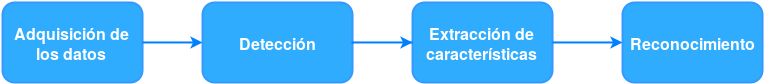
\includegraphics[scale=.6]{./Figures/MyHGR.png}
\end{center}
\caption{Metodología del sistema propuesto.}
\label{fig:MyHGR}
\end{figure}  
  
\section{Adquisición de los datos}\label{sec:KinectSensor} 

En la primera etapa del sistema los datos de entrada del sistema son capturados y preprocesados, la Figura \ref{fig:Dadquisicion} muestra este etapas de este proceso. Los datos provienen de los sensores de profundidad de dos dispositivos Kinect, debido a la naturaleza del sensor las imágenes capturadas contiene ruido por interferencia \citep{Mallick2014}, que puede ser reducido utilizando filtro de medianas \citep{Maimone2011}.

\begin{figure}[h!]
\begin{center}
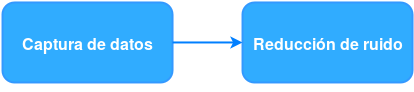
\includegraphics[scale=.6]{./Figures/Adquisicion.png}
\end{center}
\caption{Proceso de la etapa de adquisición de datos.} 
\label{fig:Dadquisicion}
\end{figure}   


\subsection{Kinect}

En noviembre del 2010 la compa\'nia Microsoft lanz\'o el sensor Kinect para consolas de vídeo juego Xbox 360 y en febrero del 2011 lanz\'o la versi\'on para Windows.   

El dispositivo Kinect esta equipado con una serie de sensores que permiten obtener imágenes a color y de profundidad (las cuales indican la distancia a la que esta ubicada un objeto del sensor. La Figura \ref{fig:KinectPic} muestra  la parte frontal del dispositivo Kinect para Windows. Los sensores permiten hacer detección y seguimiento de personas. El dispositivo tiene la capacidad de detectar hasta $6$ personas y hacer el seguimiento de hasta $2$ personas \footnote{https://msdn.microsoft.com/en-us/library/hh973074.aspx}.    
  
\begin{figure}[h!]
\begin{center}
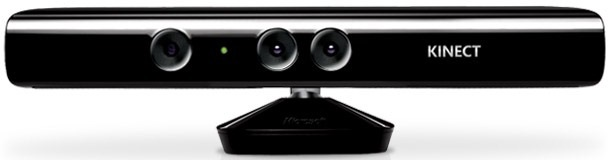
\includegraphics[scale=.65]{./Figures/Kinect.jpg}
\end{center}
\caption{Parte frontal del dispositivo Kinect en su versión para Windows, imagen recuperada de \footnotemark{}.} 
\label{fig:KinectPic}
\end{figure} 

\footnotetext{http://blogs.msdn.com/b/eternalcoding/archive/2012/02/01/official-kinect-for-windows-sdk-and-kinect-toolbox-1-1-1-are-out.aspx}

El sensor esta equipado con los siguientes componentes: un cámara de color (o sensor de color), un emisor infrarrojo, un sensor infrarrojo de profundidad, un motor que controla la inclinación, un arreglo de cuatro micrófonos y un LED, Figura\citep{Jana2013}.\\
Enseguida se describen brevemente cada uno de los componentes del sensor Kinect, estos se muestran en la Figura \ref{fig:KinectComponentes}. 

\begin{figure}[h!]
\begin{center}
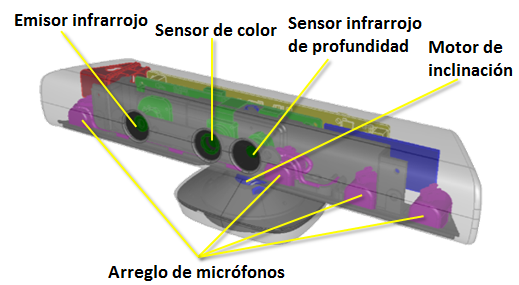
\includegraphics[scale=.6]{./Figures/sensor.png}
\end{center}
\caption{Componentes del sensor Kinect, imagen recuperada de \footnotemark{}.} 
\label{fig:KinectComponentes}
\end{figure}   

\footnotetext{https://msdn.microsoft.com/en-us/library/jj131033.aspx}

\begin{itemize}
\item La cámara de color captura y transmite datos de vídeo a color, detectando los colores rojo, verde y azul (RGB, por sus siglas en ingl\'es, red, green and blue). La transmisión de datos que brinda la cámara es una secuencia de imágenes (cuadros), a una velocidad de hasta $30$ cuadros por segundo con una resolución de hasta $1280\, x \, 960$ p\'ixeles. La velocidad de los cuadros por segundo varia según la resolución de la imagen.

\item El emisor infrarrojo proyecta puntos de luz infrarroja, estos puntos son proyectados frente al sensor. Estos puntos junto con el sensor de profundidad es posible medir la distancia que existe del sensor a algún objeto que este frente a el.  

\item El sensor infrarrojo lee los puntos infrarrojos proyectados por el emisor infrarrojo, con la lectura de los datos se calcula la distancia que existe entre el objeto y el sensor. El sensor transmite los datos de profundidad con una velocidad de hasta $30$ cuadros por segundo con una resolución de hasta $640 \, x \, 480$ pixeles.   

\item El motor de inclinación controla el \'angulo de la posición vertical de los sensores del dispositivo. El motor puede moverse desde un \'angulo de $-27^ \circ$ a $+27^\circ$, con respecto al eje vertical del sensor.  

\item La entrada de audio compuesta por un arreglo de  $4$ micrófonos permite capturar el sonido y calcular la posición de la fuente.

\item LED este indica el estado del sensor. El LED en color verde indica que el sensor esta disponible para utilizarse. El LED en color rojo indica que no existe conexión entre el Kinecy y la computadora. La ausencia de color en el LED indica que el Kinect no se encuentra conectado a la fuente de energía eléctrica.
\end{itemize}

\subsection{Filtro de mediana} 

Existen distintos métodos para eliminar el ruido por interferencia causado por dos o más  Kinect, algunos de estos métodos son invasivos pues el hardware del Kinect es modificado \citep{Mallick2014}. Una opción es utilizar filtro de mediana, pues rellena los valores faltantes en la imagen proveniente del Kinect \citep{Maimone2011}. 

Sea $Sw_{xy}$ el vecindario de tamaño $m \times n$, centrado en el pixel que se encuentra en la posición $(x,y)$. El filtro de mediana de la imagen $S(x,y)$, se calcula como: 
\begin{equation}
\^S(x,y)=\underset{(s,t)\in S_{xy}}{\text{mediana}} \lbrace S(s,t)\rbrace
\end{equation}

El filtro de mediana reemplaza el valor del pixel usando la mediana de las intensidades del vecindario del pixel, el valor del pixel en la posición (x,y) es incluido en el calculo \citep{Gonzalez2002}. 
 

%:::::::::::::::::::::::::::::::::::::::::::::::::::::::::::::::::::::::::::::::::::::::::::::::::::::::::::::::::::::::::::::::::::::::


\section{Detección}\label{sec:Detection}

En esta etapa del sistema el objetivo es localizar la mano en la imagen y segmentar la mano del fondo de la imagen. Para extraer las características necesarias para el reconocimiento.\\
Este procedimiento se lleva acabo de la siguiente manera, la Figura \ref{fig:ProcesoDeteccion} muestra el proceso para  realizar la etapa de detección. El primer paso es localizar la mano, en este trabajo se utiliza el método de detección rápida de objetos; el siguiente paso es segmentar la mano del fondo, binarizando la imagen de la mano usando el algoritmo propuesto por \citep{Otsu1979}; finalmente se aplican las operaciones morfológicas apertura y cierre, para mejorar la segmentación, es decir eliminar ruido existente. 

\begin{figure}[h!]
\begin{center}
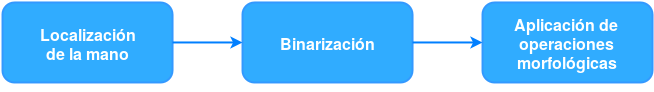
\includegraphics[scale=.7]{./Figures/Detection.png}
\end{center}
\caption{Proceso de detección de la mano.}
\label{fig:ProcesoDeteccion}
\end{figure} 

\subsection{Método detección rápida de objetos usando características simples utilizando el clasificador AdaBoost en forma de cascada}\label{subsec:ViolaJones}

En este trabajo se utiliza el método detección rápida de objetos usando características simples utilizando el clasificador AdaBoost en forma de cascada propuesto por \citep{Viola2001}, el cual fue creado originalmente para atacar el problema de detección de rostros. El método puede ser usando para detectar cualquier objeto debido a que la detección se realiza clasificando imágenes basándose en el valor de características simples.

La técnica detecta si el objeto se encuentra en la escena, usando una versión modificada del clasificador AdaBoost \citep{Freund1995} en forma de cascada, y discrimina el objeto tomando en cuenta el valor de las características Haar \citep{Viola2001}. Las características son seleccionadas usando también el clasificador AdaBoost y el valor de estas es calculado mediante el uso de una imagen integral \citep{Viola2001}. 

La Figura \ref{fig:ViolaJonesDiagram} muestra un diagrama del proceso del método de detección, el primer paso es obtener la muestras de entrenamiento con las cuales se construirá el clasificador; el siguiente paso es seleccionar las características que formarán el clasificador. Estas se escogen mediante el algoritmo de AdaBoost y su valor es calculado usando la imagen integral. El paso final  involucra construir el clasificador mediante el uso de Adaboost,  en forma de cascada.

\begin{figure}[h!]
\begin{center}
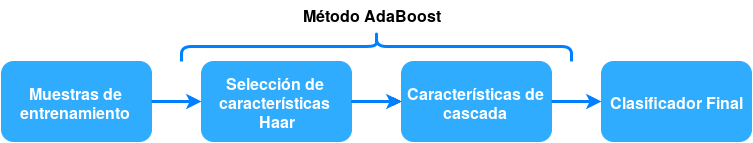
\includegraphics[scale=.6]{./Figures/ViolaJonesDiagram.png}
\end{center}
\caption{Procedimiento del algoritmo de detección rápida de objetos.}
\label{fig:ViolaJonesDiagram}
\end{figure}

Enseguida se explica a detalle cada etapa del método \citep{Viola2001}. 

\subsubsection{Características Haar}\label{sssec:CaracteristicasHaar}  

Las características Haar, son operadores rectangulares como los que se muestran en la Figura \ref{fig:haarFeatures}. A continuación se explicarán los operadores Haar básicos:
\begin{itemize}
\item Las características con dos rectángulos Figura \ref{fig:haarFeatures:1}, Figura \ref{fig:haarFeatures:2}, contienen dos regiones rectangulares adyacentes, y el valor de la característica se calcula tomando la diferencia de la suma de ambas regiones. 

\item Las características con tres rectángulos Figura \ref{fig:haarFeatures:3}, contienen tres regiones rectangulares adyacentes, y el valor de la característica se calcula sumando las regiones exteriores y restando la suma de la región interior.

\item Las características con cuatro rectángulos Figura \ref{fig:haarFeatures:4}, contienen cuatro regiones rectangulares adyacentes, y el valor de la característica se obtiene con la diferencia entre la suma de las regiones pares diagonales.
\end{itemize} 

\begin{figure}[h!]
\centering
\subfigure[]{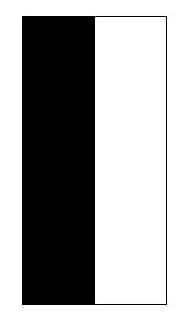
\includegraphics[scale=.4]{./Figures/haarFeatures1}\label{fig:haarFeatures:1}}
\subfigure[]{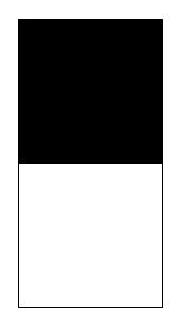
\includegraphics[scale=.4]{./Figures/haarFeatures2}\label{fig:haarFeatures:2}}
\subfigure[]{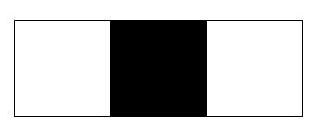
\includegraphics[scale=.4]{./Figures/haarFeatures3}\label{fig:haarFeatures:3}}
\subfigure[]{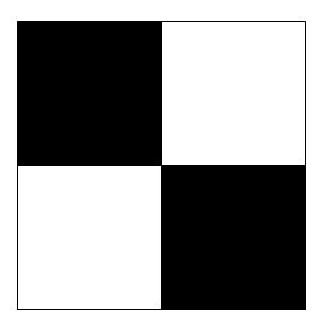
\includegraphics[scale=.4]{./Figures/haarFeatures4}\label{fig:haarFeatures:4}}
\caption{Ejemplo de tipos de operadores Haar.} \label{fig:haarFeatures}
\end{figure}


\subsubsection{Imagen integral}\label{sssec:IntegralImage} 

Uno de los aportes del método desarrollado por Viola y Jones es el concepto de imagen integral con la cual se calcula el valor de las características de manera rápida, es decir en tiempo constante, $O(1)$.  

La imagen integral, $SI$, de un imagen, $S(x,y)$, es calculada como la suma del valor de los pixeles que se encuentran arriba y a la izquierda de cierta posición de la imagen a la cual se le quiere hacer el cálculo. Lo anterior se puede escribir como: \footnote{https://computersciencesource.wordpress.com/2010/09/03/computer-vision-the-integral-image/}   
\begin{equation}
SI(x,y)=S(x,y) + S(x-1,y) + SI(x,y-1)-SI(x-1,y-1).
\end{equation}   
La Figura \ref{fig:FigIntegralImage} muestra un  ejemplo donde se calcula la imagen integral, Figura \ref{fig:FigIntegralImage:2}, de la imagen original Figura \ref{fig:FigIntegralImage:1}.
\begin{figure}[h!]
\centering
\subfigure[Imagen original]{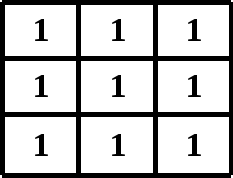
\includegraphics[scale=.6]{./Figures/ImagetoIntegral}\label{fig:FigIntegralImage:1}} \qquad
\subfigure[Imagen integral]{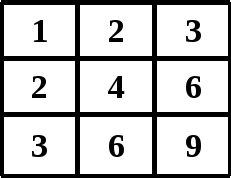
\includegraphics[scale=.6]{./Figures/CalculationIntegral}\label{fig:FigIntegralImage:2}}
\caption{Ejemplo del cálculo de la imagen integral.} 
\label{fig:FigIntegralImage}
\end{figure}

La imagen integral permite calcular la suma de los pixeles de cierta región usando solo los valores de las esquinas de la imagen integral de dicha región, la cual se obtiene como: \footnote{https://computersciencesource.wordpress.com/2010/09/03/computer-vision-the-integral-image/}    
\begin{equation}
REG(\alpha)=SI(A)+SI(D)-SI(B)-SI(C),
\end{equation}
donde $REG(\alpha)$ es la región a la cual se quiere calcular el valor de la suma de sus pixeles; $A,B,C,D$ son las esquinas de dicha región. Como se muestra en la Figura \ref{fig:figImageIntegral}, la región $\alpha$ se encuentra resaltada en color azul.  
\begin{figure}[h!]
\begin{center}
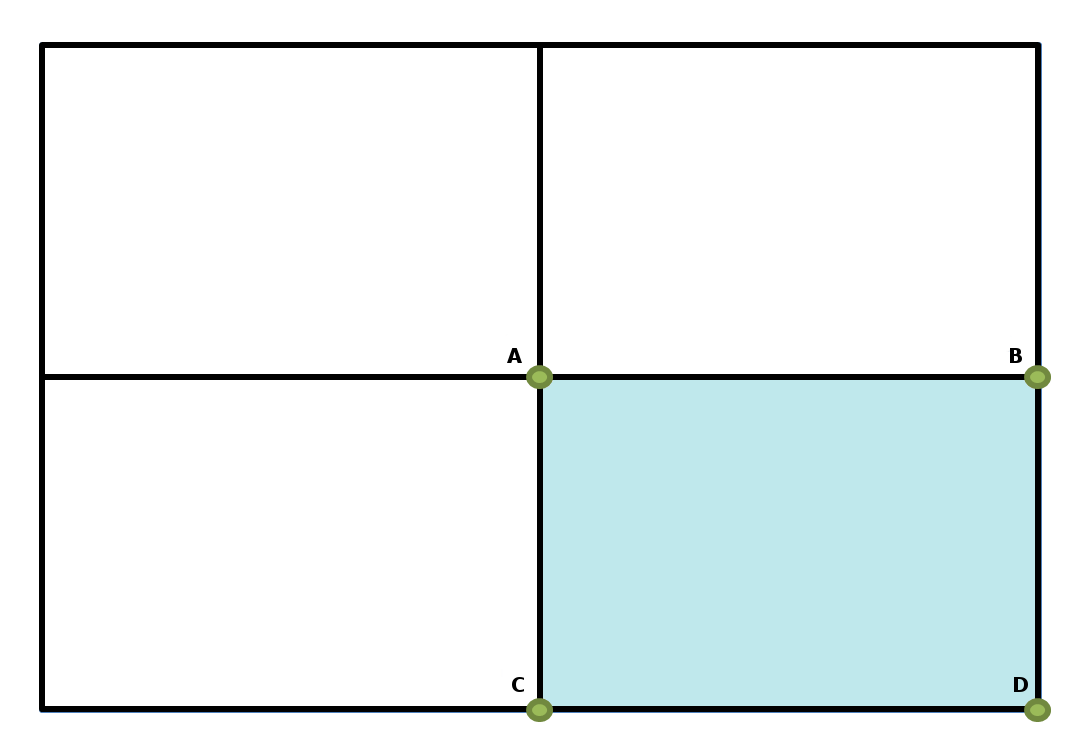
\includegraphics[scale=.25]{./Figures/IntegralImage.png}
\end{center}
\caption{Regiones de la imagen integral.}
\label{fig:figImageIntegral}
\end{figure} 


\subsubsection{Algoritmo AdaBoost}\label{sssec:AdaboostClasifier}  

En el método de detección el clasificador AdaBoost es utilizado para seleccionar las características relevantes, con las cuales se podrá detectar el objeto. También es utilizado para construir el clasificador final pero en forma de cascada, el cual es explicado en la sección \ref{sssec:AdaboostCascade}. 

El algoritmo AdaBoost realiza la discriminación de objetos construyendo un clasificador fuerte, $h(x)$, llamado así debido a que tiene una precisión mayor en comparación con los clasificadores con los que es construido, clasificadores débiles, $h_i(x)$. Los clasificadores débiles son calculados de la siguiente manera: 
\begin{equation}
h_i(x)=
\begin{cases}   
1, \quad si \quad  p_if_i(x)<p_i \theta_i \\
0, \quad de \quad otra \quad forma.\\
\end{cases} ,
\end{equation}
donde $x$ es una sub-ventana de la imagen, $f_i(x)$ es una característica, $\theta$ es un umbral, y $p_i(x)$ representa el signo de la desigualdad.   

El clasificador fuerte es una combinación lineal de los clasificadores débiles, y se define de la siguiente forma: 
\begin{equation}
h(x)= \alpha_1h_1(x)+\alpha_2h_2(x)+ \cdots +\alpha_nh_n(x) ,
\end{equation}
donde $n$ es el n\'umero de características, $\alpha_i$ es el valor asociado a cada característica, el cual va entre $0$ y $1$.

Enseguida se presenta el algoritmo AdaBoost:

\begin{algorithm}[h!]
\begin{algorithmic}[1]

\REQUIRE El conjunto $\lbrace (x_1,y_1), \cdots, (x_n,y_n) \rbrace$ donde $x_i$ representa las imágenes de entrenamiento, $y_i= 0,1,$ representa las imágenes negativas y positivas respectivamente. 
\ENSURE El clasificador fuerte $h(x)$.  

\STATE Se inicializan los pesos $w_{1,i}=\frac{1}{2m} , \frac{1}{2l},$ para $y_i=0,1$ respectivamente, donde $m$ y $l$ son el número de imágenes negativas y positivas respectivamente.  

\FOR {$t=1$ hasta $T$}   
	\STATE Se normalizan los pesos 
	$$w_{t,i}=\frac{w_{t,i}}{\sum_{j=1}^n w_{t,j}},$$ 
	para que $w_t$ sea una distribución  de probabilidad. 	
	
	\FOR {cada características $j$} 
	Entrenar un clasificador $h_j,$ donde se utiliza una sola característica. 
	El error $\epsilon$ es evaluado con respecto a $w_t$, 
	$$\epsilon = \sum_i w_i | h_i(x_i) - y_i |}.$$ 
    \ENDFOR
	
	\STATE Escoger el clasificador $h_i$ con el error más pequeño. 
	
	\STATE Se actualizan los pesos  
	$$w_{t+1,i}=w_{t,i} \beta_t^{1-e_i},$$ 
	donde $\beta_t = \frac{\epsilon_T}{1-\epsilon_t}$, el valor de  
	$e_i=0$ si $x_i$ es clasificado correctamente de otra forma $e_i=1$. 
\ENDFOR  

\STATE El clasificador final o clasificador fuerte es: 
$$ h(x) = 
\begin{cases}  
1, \quad \sum_{t=1}^T \alpha_th_t(x) \geqslant \frac{1}{2}\sum_{t=1}^T \alpha_t\\  
0, \quad de \quad otra \quad forma. 
\end{cases} ,$$
donde $\alpha_t = \log{\frac{1}{\beta_t}}$.

\caption{}\label{alg:AdaBoost}
\end{algorithmic}
\end{algorithm} 


\subsubsection{Clasificador AdaBoost en cascada}\label{sssec:AdaboostCascade}   

El objetivo de realizar la detección utilizando un clasificador en forma de cascada es descartar de manera rápida las regiones donde no se encuentra el objeto.

El clasificador en cascada  esta compuesto por etapas Figura \ref{fig:Cascade}, cada una de estas es un clasificador fuerte. Este clasificador es entrenado por medio de AdaBoost.El cual se encarga de encontrar el orden de evaluación de las características relevantes. \\
La selección se realiza como se muestra en el Algoritmo \ref{alg:Cascade} , cumpliendo cierta precisión en la detección $D$, ver Ecuación \ref{eq:D} , y cierta tasa de falsos positivos $F$, ver Ecuación \ref{eq:F} .

\begin{figure}[h!]
\begin{center}
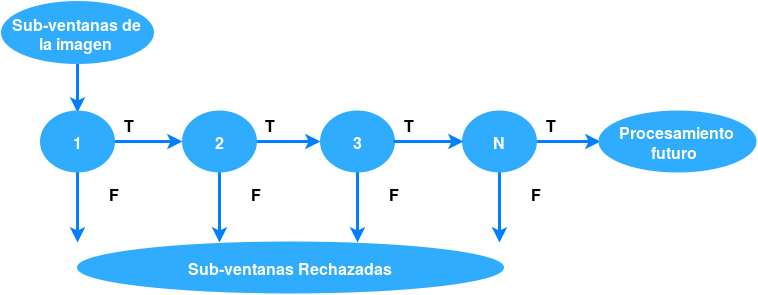
\includegraphics[scale=.60]{./Figures/DCascade.png}
\end{center}
\caption{Proceso del clasificador en forma de cascada, donde F representa la tasa de falsos positivos del clasificador de cascada y T .}
\label{fig:Cascade}
\end{figure}

El proceso de detección funciona de la siguiente manera: la sub-ventana es evaluada en el primer clasificador; un resultado positivo desencadena la evaluación de un segundo clasificador, el cual también ha sido ajustado para alcanzar cierta precisión; un resultado positivo en el segundo clasificador desencadena una tercera evaluación en el siguiente clasificador, y así sucesivamente. Un resultado negativo en cualquier punto del proceso de evaluación conduce al rechazo inmediato de la sub-ventana.

La tasa de detección del clasificador en forma de cascada es: 
\begin{equation} \label{eq:D}
D = \prod^K_{i=1} d_i ,
\end{equation}
donde $d_i$ es la tasa de precisión de detección del $i$-ésimo clasificador fuerte.  

La tasa de precisión de falsos positivos, $F$ del clasificador de cascada es: 
\begin{equation} \label{eq:F}
F = \prod^K_{i=1} f_i ,
\end{equation}
donde $K$ es el número de clasificadores fuertes y $f_i$ es la tasa de precisión del $i$-ésimo clasificador. 

\begin{algorithm}[h!]
\begin{algorithmic}[2]

\REQUIRE Imágenes positivas $P$, negativas $N$, $f$ el valor máximo de precisión de falsos positivos por etapa, $d$ es el valor mínimo de precisión en la detección por etapa. 
\ENSURE El clasificador en forma de cascada.  

\STATE  $F_0 = 1$, $D_0=1.$

\STATE  $i=0.$ 

\WHILE {$F_i > F_{Tarjet}$} 
	\STATE $i=i+1.$
	\STATE $n_i=0$, $F_i=F_{i-1}.$
	\WHILE {$F_I > F \times fp_{i-1}$} 
		\STATE $n_i = n_i +1.$ 
		\STATE Entrenar un clasificador usando AdaBoost con $P$, $N$ y $n_i$ características. 
		\STATE Evaluar el clasificador de cascada para determinar $F_i$ y $D_i$ en el conjunto de validación. 
		\STATE Decrementar el umbral para el $i$-ésimo clasificador hasta que el actual clasificador en cascada tenga un grado 			de detección de por lo menos $d \times D_i-1$.
	\ENDWHILE
	\STATE $N=0.$ 
	\IF {$F_i > F_{Tarjet}$} 
		\STATE Evaluar el actual clasificador en cascada en el conjunto de imágenes negativas y poner cualquier detección 				falsa en el conjunto $N$.
	\ENDIF

\ENDWHILE    
\caption{}\label{alg:Cascade} 
\end{algorithmic}
\end{algorithm} 


\subsection{Binarización}\label{subsec:Binarization} 

La binarización es una técnica de procesamiento de imágenes la cual se encarga de transformar una imagen en escala de grises $S(x,y)$ en una imagen binaria $B(x,y)$. Es decir los pixeles de la imagen toman un valor de $0$ ó $1$. Para formar la imagen binaria un valor o umbral de la imagen en escala de grises es seleccionado. \\ 
Una vez seleccionado el umbral, $T$, los pixeles de la imagen son discriminados. Si el valor de los pixeles de la imagen es mayor o igual al umbral entonces el valor de los pixeles de la imagen binaria es $1$, si no toma el valor de $0$. Es decir: 
\begin{equation}
B(x,y)=
\begin{cases}   
1, \quad Si \quad S(x,y)\geq T \\
0, \quad de \quad otra \quad forma\\
\end{cases}.
\end{equation}

Existen diversas técnicas para binarizar una imagen, estas se pueden clasificar en dos grupos: global y local. Los métodos globales calculan un umbral el cual es utilizado para todos los pixeles de la imagen y los métodos locales que calculan varios umbrales para ciertas regiones de la imagen \citep{Chaki2014}.  En este trabajo se utiliza el método desarrollado por \citep{Otsu1979}.

El técnica desarrolla por Otsu's es un método de binarizaci\'on global. El algoritmo asume que existen dos clases de de pixeles los del fondo y los que representan el primer plano de la imagen. El método calcula el umbral optimo $T$ que separa a estas dos clases para el cual la varianza dentro las clases es la mínima. Para calcular $T$ que minimice las varianzas dentro clases, se define como una suma ponderada de las varianzas de las dos clases.\\ 
La varianza ponderada dentro de clases es: 
\begin{equation}
\sigma^2_w(t) = q_1(t)\sigma^2_1(t) + q_2(t)\sigma^2_2(t),
\end{equation} 
donde las probabilidades de cada clase son calculadas mediante:  
\begin{equation}
q_1(t) = \sum ^t_{i=0} P(i) 
\qquad \text{y} \qquad
q_2(t) = \sum ^{255}_{i=t+1} P(i),
\end{equation} 
y la media de cada clase es calculada como:  
\begin{equation}
\mu_1(t) = \sum ^t_{i=0} \frac{i \cdot P(i)}{q_1(t)} 
\qquad \text{y} \qquad
\mu_2(t) = \sum ^{255}_{i=t+1} \frac{i \cdot P(i)}{q_2(t)}.
\end{equation} 
\\
La varianza total $\sigma^2$, es igual a la suma de la varianza dentro de clase y la varianza entre clases $\sigma^2_b(t)$, es decir: 
\begin{equation}
\sigma^2 = \sigma^2_w(t) + \sigma^2_b(t),
\end{equation}
donde $\sigma^2_b(t)= q_1(t)\left[ 1- q_1(t) \right]\left[ \mu_1(t) - \mu_2(t) \right]^2 .$  \\
Como la varianza total no depende de $t$, es una constante, entonces para encontrar el umbral que minimice la varianza dentro de clases equivale a encontrar el máximo de $\sigma^2_b(t)$. 

\subsection{Operaciones Morfológicas}\label{subsec:OperacionesMorfologicas} 

Otra técnica muy utilizada en procesamiento de imágenes son las operaciones morfológicas.Que son un conjunto de operaciones no lineales. La idea es que al aplicar alguna de estas operaciones el ruido sea removido tomando en cuenta la forma y estructura de la imagen.\\ 
Las operaciones morfológicas \citep{Premaratne2013} utilizan un elemento estructural el cual se aplica por toda la imagen. Los elementos estructurales pueden ser de distintas formas como los que se muestran en la Figura \ref{fig:EX}.
\begin{figure}[h!]
\centering
\subfigure[Rectángulo de $3x3$.]{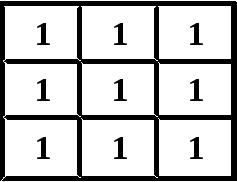
\includegraphics[scale=.68]{./Figures/EX1}\label{fig:EX:1}} \qquad
\subfigure[Figura de $3x2$.]{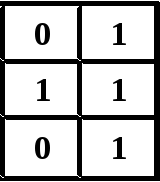
\includegraphics[scale=.68]{./Figures/EX3}\label{fig:EX:3}} \qquad
\subfigure[Cruz de $5x5$.]{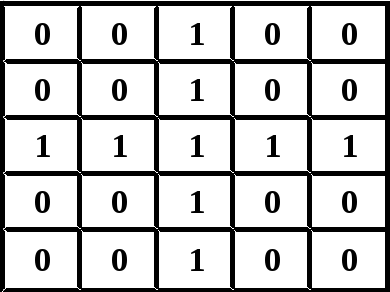
\includegraphics[scale=.42]{./Figures/EX2}\label{fig:EX:2}} 
\caption{Ejemplos de elementos estructurales.} \label{fig:EX}
\end{figure} 

Existen distintas operaciones morfológicas, las básicas o principales son la dilatación y erosión las cuales se explican enseguida junto con la apertura y cierre. 
 
\subsubsection{Dilatación}\label{sssec:Dilatation}
La dilatación es una operación que añade pixeles a la orilla de los objetos que se encuentran en la imagen. En la Figura \ref{fig:OM:2} 
se aplica esta operación a la Figura \ref{fig:OM:1}.\\
La dilatación se define como:  
\begin{equation}
S \oplus EX = \lbrace S|EX_S \subseteq S \rbrace,
\end{equation}
donde $EX_S$ es el elemento estructural trasladado con la imagen. 

\subsubsection{Erosión}\label{sssec:OMerosion}
La erosión remueve pixeles a la orilla de los objetos que se encuentran en la imagen. En la Figura \ref{fig:OM:3} se muestra el resultado de aplicar la operación a la Figura \ref{fig:OM:1}.\\ 
La erosión se define como: 
\begin{equation}
S \ominus EX = \lbrace S|EX_S \subseteq S \rbrace,
\end{equation}
donde $EX_S$ es el elemento estructural trasladado con la imagen. 

\subsubsection{Apertura}\label{sssec:Opening} 
La operación apertura abre huecos entre objetos conectados por un enlace delgado de pixeles, también suaviza los contornos del objeto. Esta operación se calculada realizado dos operaciones básicas una erosión seguida de una dilatación \\ 
La apertura se define como:  
\begin{equation}
S \circ EX = (S \ominus EX) \oplus EX.
\end{equation}
La Figura \ref{fig:OM:4} muestra el resultado de aplicar la operación apertura a la Figura \ref{fig:OM:1}.

\subsubsection{Cierre}\label{sssec:Closure}
La operación cierre elimina huecos pequeños y rellena huecos en los contornos. El cierre es calculado realizando las operación de dilatación seguida de la erosión.\\
El cierre se define como:
\begin{equation}
S \bullet EX = (S \oplus EX) \ominus EX.
\end{equation}
La Figura \ref{fig:OM:5} muestra el resultado de aplicar la operación a la Figura \ref{fig:OM:1}.

\begin{figure}[h!]
\centering
\subfigure[original]{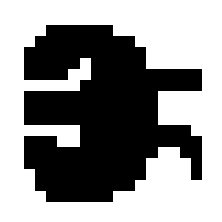
\includegraphics[scale=.55]{./Figures/originalMO}\label{fig:OM:1}} \hspace{10mm}
\subfigure[dilatación]{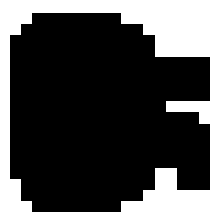
\includegraphics[scale=.55]{./Figures/dilatationMO}\label{fig:OM:2}} \hspace{10mm}
\subfigure[erosión]{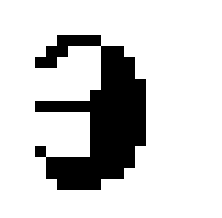
\includegraphics[scale=.55]{./Figures/erosionMO}\label{fig:OM:3}} \hspace{10mm}
\subfigure[apertura]{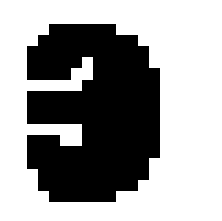
\includegraphics[scale=.55]{./Figures/openingMO}\label{fig:OM:4}} \hspace{10mm}
\subfigure[cierre]{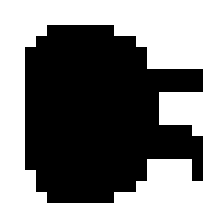
\includegraphics[scale=.55]{./Figures/closingMO}\label{fig:OM:5}}
\caption{Aplicación de las principales operaciones morfológicas a la imagen que se encuentra en el inciso a, \citep{Smith1999}.\quad }\label{fig:OM}
\end{figure} 




%:::::::::::::::::::::::::::::::::::::::::::::::::::::::::::::::::::::::::::::::::::::::::::::::::::::::::::::::::::::::::::::::::::


\section{Extracción de características}\label{sec:Convexhull} 

La finalidad de esta etapa es obtener las características de la imagen que sean capaces de describir la mano, de manera que con estas, se pueda reconocer los gestos realizados.
   
En este trabajo se extraen características geométricas, las cuales son extraídas de la siguiente forma, ver Figura \ref{fig:DiagramaExtraccionCaracteristicas}: el primer paso es encontrar la envolvente convexa de la mano para posteriormente calcular los defectos de convexidad, una vez aplicados estos algoritmos se calcula el número de dedos de la mano entre otras características; finalmente las características calculadas  se guardan en un vector.  

\begin{figure}[h!]
\begin{center}
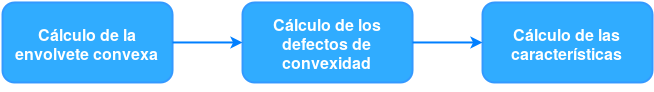
\includegraphics[scale=.7]{./Figures/DExtraccion.png}
\end{center}
\caption{Proceso de la extracción de características.}
\label{fig:DiagramaExtraccionCaracteristicas}
\end{figure} 

A continuación se definen los conceptos anteriores y el de conjunto convexo.

Sea $A$ un conjunto en el espacio euclidiano $\bold{\Re}^d$, donde $d$ es la dimensión del espacio euclidiano. $A$ es un conjunto convexo \footnote{\label{ConvexFN} Weisstein, Eric W. "Convex." From MathWorld--A Wolfram Web Resource. http://mathworld.wolfram.com/Convex.html} si contiene todos los segmentos de línea que unen a cualquier par de puntos pertenecientes al conjunto.  
\begin{figure}[h!]
\centering
\subfigure[Convexo]{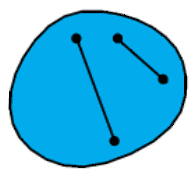
\includegraphics[scale=.8]{./Figures/ConvexSet.png}\label{fig:Sets:Convex}} \hspace{10mm}
\subfigure[conexo]{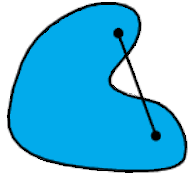
\includegraphics[scale=.75]{./Figures/ConcaveSet.png}\label{fig:OM:Concave}} \hspace{10mm}
\caption{Ejemplo de un conjunto conexo y un convexo. Image recuperada de \ref{ConvexFN} }\label{fig:Sets}
\end{figure} 

Sea $B$ un conjunto de puntos en el plano Euclidiano, la envolvente convexa de $B$ es el conjunto convexo más pequeño que contiene a todos los puntos en $B$. En la Figura \ref{fig:FigConvexHullDefects} se muestra de color rojo la envolvente convexa de la Figura cuyo contorno se encuentra de color negro. 

Los defectos de convexidad de la envolvente convexa, son el conjunto de puntos que no pertenecen al casco convexo. El defecto es el espacio que existe entre el contorno de la envolvente convexa y del objeto.\\
Sea $CD=\lbrace cd_1, cd_2, \cdots, cd_n \rbrace$ el conjunto de defectos de convexidad de una envolvente convexa. Cada defecto esta compuesto por tres elementos: el punto de inicio del defecto $s_i(x,y)$, el punto con mayor distancia de la envolvente al objeto, $d_i(x,y)$ y el punto final del defecto, $e_i(x,y)$.
En la Figura \ref{fig:FigConvexHullDefects} los puntos amarillos representan los puntos de profundidad de los defectos de convexidad. 

\begin{figure}[h!]
\begin{center}
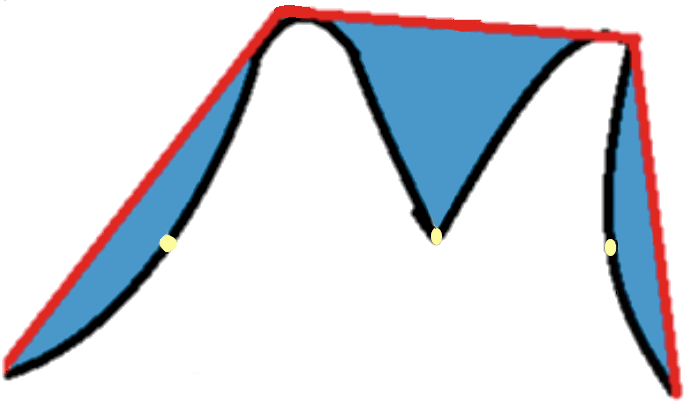
\includegraphics[scale=.4]{./Figures/ConvexHullAndDefects.png}
\end{center}
\caption{En la imagen se aprecia de color rojo la envolvente convexa, de negro el contorno de la Figura, y los puntos amarillos son el punto de profundidad de los defectos de convexidad.}
\label{fig:FigConvexHullDefects}
\end{figure}  

Usando las técnicas anteriores podemos extraer características importantes como el número de dedos, la posición del centro de la palma de mano, la posición de la punta de los dedos, la posición del inicio o raíz de los dedos, el ángulo del centro de la palma de la mano a la punta de los dedos, ángulo $TC$, el ángulo del centro de la palma de la mano a al inicio de los dedos, ángulo $RC$ y la distancia vertical del centro de la palma de la mano al inicio de los dedos. Enseguida se explica como son obtenidas las características mencionadas. 

El número de dedos que se encuentran levantados es calculado con el Algoritmo \ref{alg:NumDedos} desarrollado por \citep{Kathuria2011}, el cual utiliza los defectos de convexidad en especifico los conjuntos de puntos de inicio, $\mathcal{S}=\lbrace s_1(x,y), s_2(x,y), \cdots, s_n(x,y) \rbrace$, los puntos de mayor distancia, $\mathcal{D}=\lbrace d_1(x,y), d_2(x,y), \cdots, d_n(x,y) \rbrace$, las distancias del punto de inicio al de mayor distancia, $\mathcal{\delta}=\lbrace \delta_1(x,y), \delta_2(x,y), \cdots, \delta_n(x,y) \rbrace$, donde $n$ es el número total de defectos de la envolvente convexa .\\
Sea $C_r(x,y)$, el punto que representa el centroide del rectángulo más pequeño que encierra a la mano, $L_r$, la altura del rectángulo y $k$ una constante. 

\begin{algorithm}[h!]
\begin{algorithmic}[1]
\REQUIRE Los conjuntos $\mathcal{S}$, $\mathcal{D}$, el punto $C_r$ y el valor $L_r$.   
\ENSURE Número de dedos levantados, $Nf$.  
\FOR{$i=1$ hasta $n$}  
	\STATE $k=6$. 	
	
	\IF{$ \left[ s_i(x,y) < C_r(x,y)$ \textbf{O} $d_i(s,y) < C_r(x,y) ]$ \textbf{Y} $s_i(x,y) < d_i(x,y)$ \textbf{Y} $ \delta_i > \frac{L_r}{k}$ } 
	\STATE $Nf=Nf+1$
	\ENDIF 
\ENDFOR 

\caption{Cálculo del número de dedos levantados de la mano.}
\label{alg:NumDedos} 
\end{algorithmic}
\end{algorithm} 

La posición de la raíz de los dedos, $Fr(s,y)$ puede ser calculada usando los defectos de convexidad \citep{Hummel2014}, en especifico los puntos de profundidad, $d(x,y)$. Se calcula tomando el punto medio de los puntos de profundidad consecutivos encontrados en medio de los dedos, como se muestra en la Figura \ref{fig:RootFingers} . Es decir: 
\begin{equation}
Fr_i(x,y)= \left( \frac{ x_{d_i}+x_{d_{i-1}} }{2},\frac{y_{d_i}+y_{d_{i-1}}}{2}  \right),
\end{equation}

donde $i$ representa el número de dedo, cuando $i=0$ se toma el punto de profundidad anterior al dedo, si $i=6$ se toma el punto de profundidad posterior al dedo. 

\begin{figure}[h!]
\begin{center}
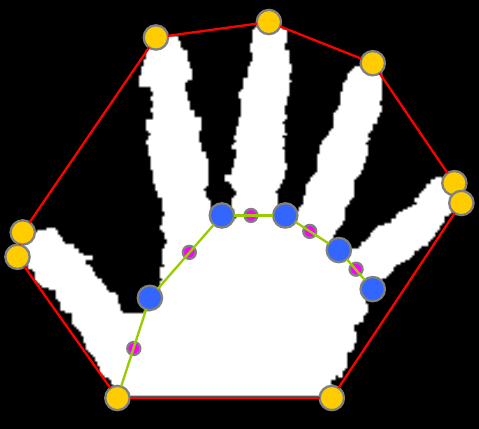
\includegraphics[scale=.55]{./Figures/rootFingers.png}
\end{center}
\caption{La Figura muestra parte de la mano y en ella se aprecia los siguientes elementos: en color rojo la envolvente convexa, en amarillo los puntos de inicio y final de los defectos de convexidad,  en color azul los puntos de profundidad de los defectos, en verde la linea que une a los puntos de profundidad consecutivos y finalmente en morado los puntos medios, \citep{Hummel2014}} 
\label{fig:RootFingers}
\end{figure} 

El centro de la palma de mano también es calculado, con los puntos de profundidad de los defectos de convexidad, para ello se toma como centro de la palma el centro del rectángulo mas chico que une rodea a los puntos de convexidad. 

El ángulo $RC$ es el formado por el eje $y$  y la línea que une al punto que representa la posición de la raíz de los dedos, $Fr(x,y)$ con el centro de la palma de la mano, $Ch(x,y)$, \citep{Sgouropoulos2014}. 
\begin{equation}
\angle RC = 90^\circ - \tan^{-1} \left( \frac{ y_{Fr}-y_{Ch} }{ x_{Fr}-x_{Ch} } \right).
\end{equation}


El ángulo $TC$ es el formado por el eje $y$ y la línea que une al centro de la mano, $Ch(x,y)$ y con el de la punta de los dedos, $Ft(x,y)$, \citep{Sgouropoulos2014}. El  ángulo anterior se representa como:
\begin{equation}
\angle TC = 90^\circ - \tan^{-1} \left( \frac{ y_{Ft}-y_{Ch} }{ x_{Ft}-x_{Ch} } \right).
\end{equation}
 

La distancia $PC$ es la distancia vertical de la raíz del dedo al centro de la palma de la mano. Esta distancia es invariante al tamaño de la mano ya que es dividida por el tamaño de la palma, que se toma como el ancho del rectángulo que encierra la palma.  

\begin{figure}[h!]
\begin{center}
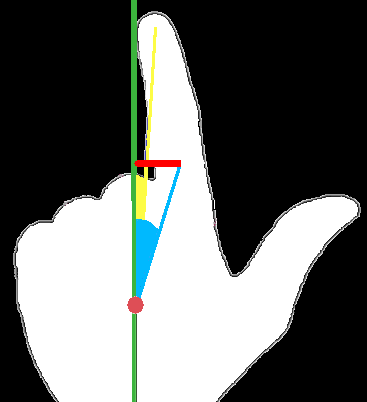
\includegraphics[scale=.6]{./Figures/angles.png}
\end{center}
\caption{En la imagen se representan los siguientes elementos, el eje vertical con respecto a la mano se encuentra como una línea de color verde; la línea roja represente la distancia del eje vertical a la raíz de los dedos; el punto rosa representa el centro de la palma de la mano, el área azul representa el ángulo de que existe de la línea que una al centro con la raíz de los dedos y finalmente el área amarilla representa el ángulo que forma la línea del centro a la punta de los dedos, \citep{Sgouropoulos2014}.}
\label{fig:anglesFingers}
\end{figure} 


Una vez que todas las características son calculadas estas son guardadas en un vector, llamado vector de características. La dimensión del vector es el número de características que este contiene. 


%:::::::::::::::::::::::::::::::::::::::::::::::::::::::::::::::::::::::::::::::::::::::::::::::::::::::::::::::::::::::::::::::::


\section{Reconocimiento}\label{sec:SVM} 

Es la etapa final del reconocimiento, es donde el gesto realizado por el usuario finalmente puede ser interpretado por la computadora.\\  
En este trabajo el reconocimiento se realiza utilizando el algoritmo de máquinas de soporte vectorial SVM, por sus siglas en ingles \citep{Cortes1995}, un método de aprendizaje de máquina supervisado el cual es utilizado para resolver problemas de clasificación y regresión. SVM tiene como objetivo crear un modelo basado en datos conocidos, datos de entrenamiento, donde este modelo es capaz de predecir a que clase pertenecen datos nuevos. 

SVM realiza la clasificación separando las clases calculando el hiperplano que tengan el margen de separación más grande. En la Figura \ref{fig:SVM} se muestra en conjunto de clases separables por medio de un hiperplano .  

\begin{figure}[h!]
\begin{center}
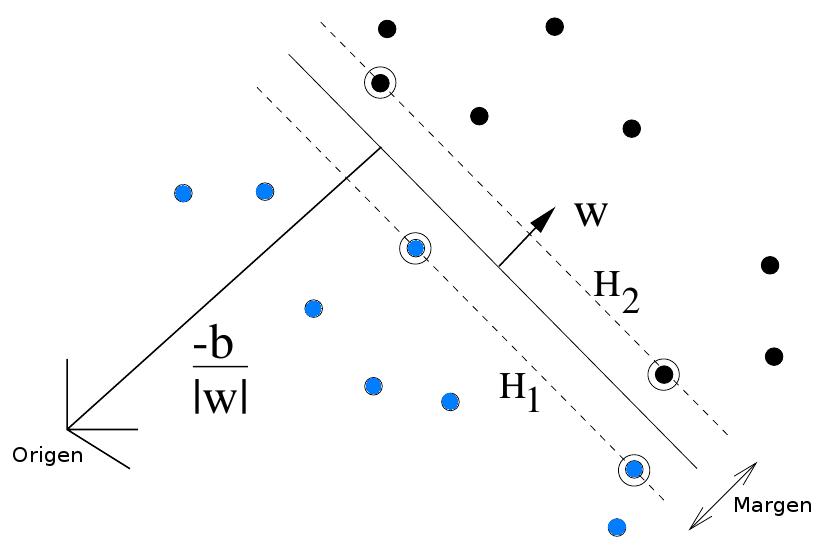
\includegraphics[scale=.55]{./Figures/SVMarticle.png}
\end{center}
\caption{La imagen muestra la separación de dos clases, (los círculos en color azul y negro), mediante un hiperplano óptimo; donde $\textbf{w}$ representa la normal al hiperplano, $\frac{\textbf{-b}}{\textbf{w}}$ la distancia el hiperplano al origen. \citep{Burges1998}.}
\label{fig:SVM}
\end{figure} 

Enseguida se explica el caso cuando las clases son linealmente separables.\\
Dado $N$ muestras de entrenamiento $x_i$, de dimensión $D$, dos clases distintas $y_i=-1$ ó $+1$ es decir: 
$$\lbrace x_i,y_i \rbrace \quad \text{donde} \quad  i=1, \cdots ,N \quad y\in \lbrace -1,1 \rbrace \quad x \in \Re^D.$$
Sea  
\begin{equation}\label{eq:hiper}
w \cdot x + b = 0 ,
\end{equation}  
el hiperplano óptimo que separa a las clases, donde $w$ es la normal al hiperplano, $\frac{b}{ \Vert w \Vert}$ es la distancia perpendicular desde el hiperplano al origen.

Sea $d_+$, la menor distancia del hiperplano que separa a las muestras positivas de las negativas y $d_-$, la menor distancia del hiperplano que separa a las muestras negativas de las positivas. Se define el margen del hiperplano como la suma de estas distancias, es decir: $d_+ + d_-$.

Para el caso cuando las clases son linealmente separables basta con encontrar el hiperplano con el margen mayor. Es decir que el hiperplano puede ser calculado seleccionando $w$ y $b$ de manera que los datos de entrenamiento cumplan con:  
\begin{equation}\label{eq:des+1}
w \cdot x_i + b \geqslant +1 \quad \textrm{ para } \quad y_i=+1
\end{equation} 
\begin{equation}\label{eq:des-1}
w \cdot x_i + b \leqslant -1 \quad \textrm{ para } \quad y_i=-1
\end{equation} 
Combinando las desigualdades anteriores, se obtiene:  
\begin{equation}
y_i(x_i \cdot w + b) -1 \geqslant 0 \qquad \forall i 
\end{equation} 

Tomando en cuenta los puntos en donde se cumple la igualdad de la Ecuación \ref{eq:des+1}. Estos puntos se encuentran sobre el hiperplano $H_1$, el cual se escribe como: 
\begin{equation}\label{eq:eq+1}
w \cdot x_i + b = +1,  
\end{equation} 
con normal $w$ y una distancia perpendicular desde el origen de $\frac{\vert 1-b \vert}{ \Vert w \Vert}$. 
Similarmente para la Ecuación \ref{eq:des-1}, entonces el hiperplano $H_2$ se describe como: 
\begin{equation}\label{eq:eq+1}
w \cdot x_i + b = -1,  
\end{equation} 
con normal $w$ y una distancia perpendicular desde el origen de $\frac{\vert-1-b\vert}{ \Vert w \Vert}$.\\ 
Como $d_+ = d_- = \frac{1}{\Vert w \Vert}$, el margen es $\frac{2}{\Vert w \Vert}$. Los hiperplanos son paralelos pues tienen la misma normal, también ninguna muestra de entrenamiento caen entre ellos. Entonces se puede encontrar un par de hiperplanos  que tengan un margen máximo minimizando $\Vert w \Vert^2$, es decir:  
\begin{equation}
\text{min} \quad \frac{1}{2} \Vert w \Vert \quad \text{tal que} \quad y_i(w \cdot x_i + b) -1 \geq 0.
\end{equation}  




\newpage
%%=====================================================
